\chapter{試作2号機:インスタンス認識ハンド}
\newpage

\section{要求仕様}
1号機の課題の中で特に,自由度が少ない点と物体を識別できない点は日常生活で使用する上で必須である.そこで2号機ではこれら2点の課題を克服したロボットハンドを開発する.

1号機では対象に近づきグリップすることのみを行ったが,実応用を考えると物を持って何かをする必要が出てくる.そこで2号機では手首に重点を置き,より多彩な動きを実現するためアクチュエータを増やした.スマホでは環境を認識するのに1秒程かかってしまい,より高速に演算できる必要がある.また多くのアクチュエータを制御するため,スマホではなくPCで学習・推論を行うように変更した.

物体をピックアップするために物体との距離を捉える必要がある.

自由度

点で掴む,真ん中で掴む,掴んだ後に滑りを防ぐ必要

掴む時の把持点決定及び指定した点を掴むモータ調整


\section{機構設計・機体デザイン}

対象物との距離を測るためにデプスカメラを用いる.


対象物を持ち上げるために腕に関節を1つ加え,地面から垂直に持ち上げられるようにした.

タイヤによる把持点制御では移動方向が回転方向になるため制御が難しい.
対象物の把持点を調整するために,腕を進行方向と垂直な方向にスライドできるよう,ラック\&ピニオンを用いてサーボモータの回転を水平移動にした.

把持点を正確に掴むために,手は把持点に対して対称に掴むよう設計した.

% 向きの定義(x軸,y軸,z軸)


\section{制御アルゴリズム}
2号機では強化学習ではなく比例制御の考え方を利用した手法及びルールベースによって対象物のピックアップを行う.

接近動作では2段階に分けて行う.まず対象物までのラフな接近について述べる.
対象物のマスクを取得し重心を計算する.その重心がロボットハンドの中心軸に来るように左右輪のスピードをそれぞれ独立に以下の更新式によって制御しながら接近する.

\begin{lstlisting}[label=code:motor]
    r_motor = (1 - error_distance) / 2 * MAX_SPEED
    l_motor = (1 + error_distance) / 2 * MAX_SPEED
\end{lstlisting}

ここで\texttt{MAX\_SPEED}はモーターの最大スピードで今回は100とした.\texttt{error\_distance}はロボットハンドと対象物との画像内におけるx軸方向のズレを画像の横の長さで規格した値であり,-1から1の値をとる.そして対象物から20cmまで近づいたら停止させる.

次に,対象物の重心にハンドの把持中心が来るように横方向にラックピニオンで修正を加える.この時,画像におけるピクセル間距離を実距離に変換し重心とハンド中心の変位をなるべく小さくするようにサーボを動かす.そしてデプスカメラが対象物に覆われて見えなくなるまで直進する.
そこからさらに4cm直進しグリッパーを閉じる.その後腕を上げ物体を持ち上げ,この際のデプス画像を保持しておく.そこから1秒ごとにデプス画像の現フレームとのピクセル数比を取り,50\%以下であったら失敗とし,5秒落とさず維持したら把持成功とした.


\subsection{シリアル通信における情報圧縮}
Arduinoとのシリアル通信では1回に2byteまでしか送信できず,Stringでモーター5つの情報を送信すると遅延や読み飛ばしが発生した.そこで2号機ではモーターの取る値をデジタル化し情報を圧縮した.



% \subsection{色抽出}



\subsection{デプスカメラを使用したカメラ画像内における実距離推定}
把持位置を制御する際,画像内の実際の長さ知る必要がある.そこで,ピクセル間距離から実距離を回帰処理によって求めた.また,カメラから測る対象物までの距離にも依存するため,デプスカメラを用いて距離依存性についても回帰処理を行い,2段階で求めた.

壁に30cm定規を置き,カメラは壁と平行になるよう設置した.壁からカメラの距離$z$(cm)を変えながら定規の目盛りのピクセル座標を取得し,横軸にピクセル差分$\Delta \rm{pixel}$,縦軸にそのピクセルに対応する定規の目盛り幅$\Delta x$(cm)をプロットした(\fig{pix2dist}).また,各$z$で線形回帰を行ったあと横軸に壁からカメラの距離$z$,縦軸に傾き$a$をプロットし線形回帰を行い,全ての距離$z$におけるピクセル間距離を求めた(\fig{depth2grad}).


\begin{figure}[H]
    \centering
    \begin{minipage}{0.45\columnwidth}
        \centering
        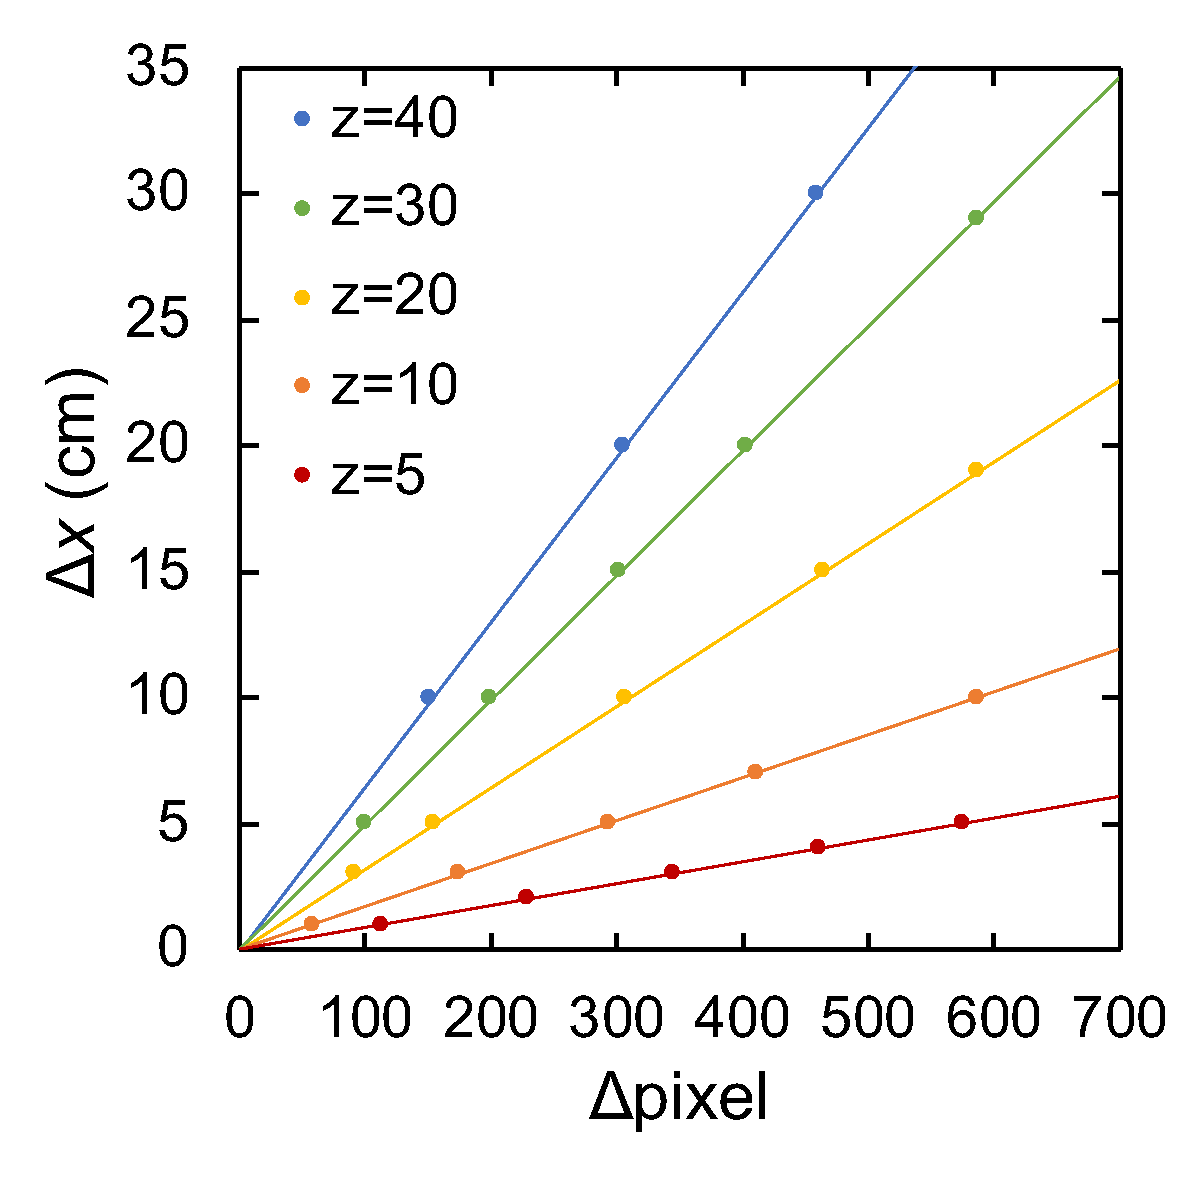
\includegraphics[width=\linewidth]{figure/chapter4/pixel2distance}
        \subcaption{Pixel to Distance}
        \label{fig:pix2dist}
    \end{minipage}
    \begin{minipage}{0.45\columnwidth}
        \centering
        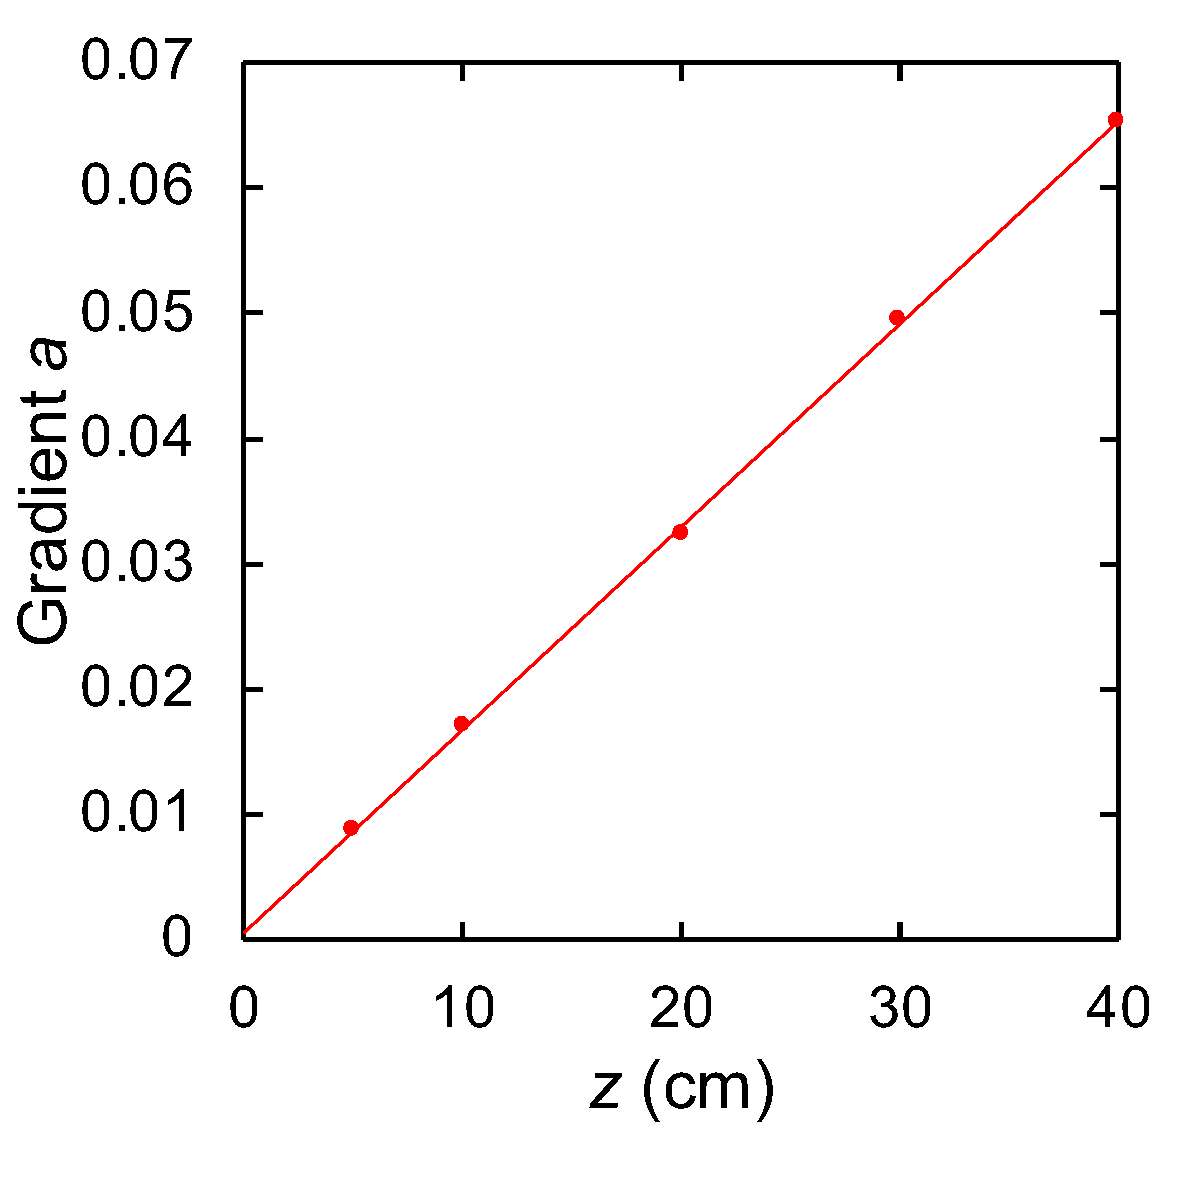
\includegraphics[width=\linewidth]{figure/chapter4/depth2gradient}
        \subcaption{Dependency of depth}
        \label{fig:depth2grad}
    \end{minipage}
    \caption{Convert pixel-wise to distance in real.}
    \label{fig:pix2distance}
\end{figure}
\begin{figure}[H]
    \centering
    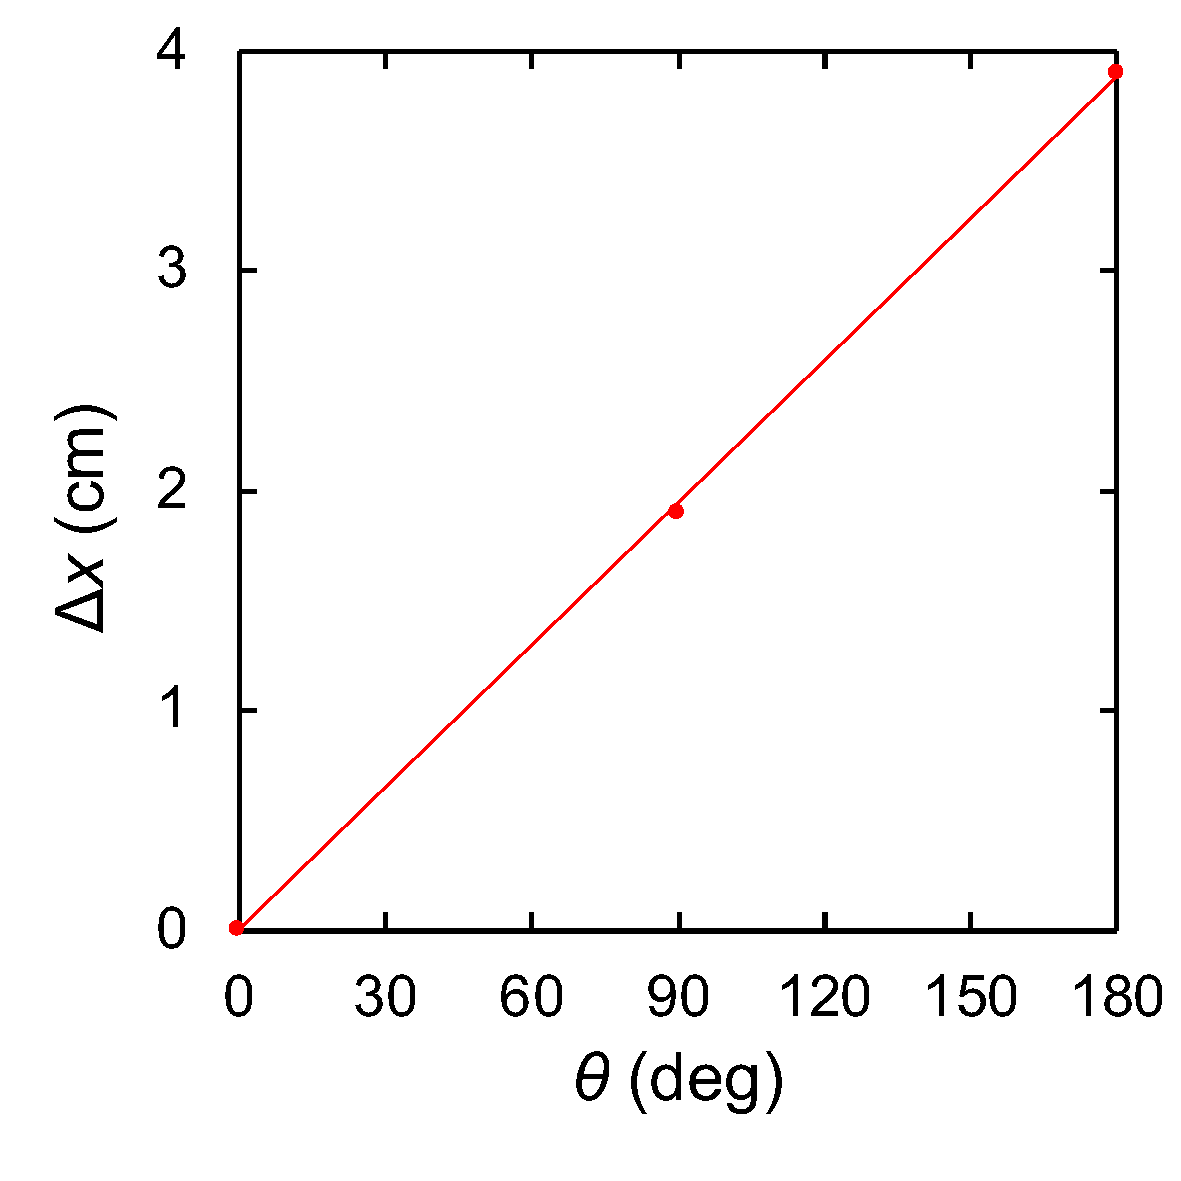
\includegraphics[width=0.5\linewidth]{figure/chapter4/servo2distance}
    \caption{Convert servo input to distance.}
    \label{fig:servo2dist}
\end{figure}

以上から,実距離$\Delta x$はピクセル間距離$\Delta \rm{pixel}$とカメラと対象物の距離$z$を用いて
\begin{align}\label{eq:ピクセル間距離}
    \Delta x \simeq (0.0016z + 0.0006) \cdot \Delta \rm{pixel}
\end{align}
と推定できる.

また,ラック\&ピニオンの回転から水平移動に変換するためには,サーボが0\deg -- 180\deg まで可動するため,その移動最大距離を測定しておき(4cm),各角度における0\deg からの移動量をプロットし線形回帰する(\fig{servo2dist})ことで以下のように求められる.

\begin{align}\label{eq:スライド角度}
    \Delta x \simeq 0.0216 \theta
\end{align}
ここで,$\Delta x$は水平移動距離(cm),$\theta$はサーボの回転角度(deg)である.
\eq{ピクセル間距離}と\eq{スライド角度}から
\begin{align}
    \theta & \simeq \dfrac{\Delta x}{0.0216} \\
           & = \dfrac{0.0016z + 0.0006}{0.0216} \Delta \rm{pixel} \\
\end{align}
として画像からサーボを何度動かせば良いかが分かる.なお,実装上はサーボの可動範囲が0\deg -- 180\deg を考慮して
\begin{lstlisting}[label=code:servo]
    vertical_deg =\
        (max(min(vertical_pos // 0.0216, 90), -90) + 90) // 10
\end{lstlisting}
とすることで入力の最小0,最大を180とし,サーボへの入力が0の時に真ん中である90\deg とし,それを1/10にデジタル化して送信する.\texttt{vertical\_pos}は$\Delta x$(cm),\texttt{vertical\_deg}は$\theta$(deg)である.


\subsection{Mask R-CNNを用いた物体のセグメンテーションと測距}
Instance Segmentationの手法の1つであるMask R-CNNを用いた.MSCOCO2014および2017のデータセットで学習した.
学習した結果を\tab{MSCOCO評価}に示す.

\begin{table}[H]
    \centering
    \caption{Results of Mask R-CNN validated by COCO.}
    \begin{tabular}{ccccc}\toprule
        & \multicolumn{2}{c}{Object Detection} & \multicolumn{2}{c}{Segmentation} \\ 
         & 2014 & 2017 & 2014 & 2017 \\ \midrule
        $\rm{AP}^{\rm{IoU}=0.50:0.95} \u{maxDets=100} @Area=all$ & 0.352 & 0.227 & 0.334 & 0.243 \\ 
        $\rm{AR}^{\rm{IoU}=0.50:0.95} \u{maxDets=100} @Area=all$ & 0.438 & 0.299 & 0.405 & 0.301 \\ 
        FPS & 4.078 & 3.880 & 4.013 & 4.002 \\ \bottomrule
    \end{tabular} 
    \label{tab:MSCOCO評価}
\end{table}

また,デプスカメラを用いて検出した物体の距離も同時に測定した.Mask R-CNNの出力であるマスクの重心を求め,その座標までの距離をデプスカメラで測定した.\fig{maskrcnn例}に学習済みモデルを使用した物体検出およびその物体までの測距の例を示す.



このように,マスクが完璧出なくとも対象物の重心はおおよそ把握できるため,IoUよりもPrecisionを重視し物体検出におけるFPSが高い2014年学習モデルを使う.


\section{評価}
今回2号機でアップデートしたのは,対象物の識別と把持動作であったため,この2点に関して評価を行う.

MSCOCOデータセットの中で,机の上にあるものを把持できるかを検証した.
今回,対象とした物体は以下の4点である.
\begin{itemize}
    \item bottle
    \item cup
    \item cell phone
    \item apple
\end{itemize}

まず,学習済みモデルを使用して識別精度の対象物との距離依存性を検証した.



\section{まとめ}
物体の種類を識別し,把持し,元の位置に持ち帰ることができた.



